\documentclass[11pt,a4paper]{article}

\usepackage{epsfig}
\usepackage{multicol}

\usepackage[utf8]{inputenc}
\usepackage[brazil]{babel}
\usepackage{fancyheadings}
\usepackage{amsmath}
\usepackage{calrsfs}
\usepackage{enumerate}
\usepackage{enumitem}   
\DeclareGraphicsExtensions{.png,.pdf}
\usepackage{amsmath, amsfonts, amssymb}
\usepackage{esint}
\usepackage{graphicx}
\usepackage{multicol}
\usepackage{tasks}
\usepackage[utf8]{inputenc}
\usepackage{mathrsfs} % Transformada de Laplace
\usepackage{indentfirst}

% As margens
\setlength{\textheight}{24.0cm}
\setlength{\textwidth}{17.5cm}
\setlength{\oddsidemargin}{2.0cm} % Margens reais desejadas
\setlength{\evensidemargin}{2.0cm} % 2+17.5+1.5=21cm (largura A4)
\setlength{\topmargin}{1.5cm} % 1.5+1.6+1.0+24.0+1.6=29.7cm
\setlength{\headheight}{1.6cm} % (altura A4)
\setlength{\headsep}{1.0cm}
\setlength{\columnsep}{1.5cm} % Coluna = 8cm ((17.5-1.5)/2)
\addtolength{\oddsidemargin}{-1in}
\addtolength{\evensidemargin}{-1in}
\addtolength{\topmargin}{-1in}
\setlength{\footskip}{0.0cm}


% Novos comandos
\newcommand{\limite}{\displaystyle\lim}
\newcommand{\integral}{\displaystyle\int}
\newcommand{\somatorio}{\displaystyle\sum}
\newcommand{\mat}[1]{\mbox{\boldmath{$#1$}}} 

\pagestyle{fancy}


\usepackage{lipsum}

\lhead{

\includegraphics[width=1cm]{brasao.png}
}

\rhead{ 
\sc\textbf{U}niversidade \textbf{F}ederal do \textbf{C}eará\\
Campus Quixadá\\ Monitoria de Cálculo II, III e EDO}

\cfoot{}

\begin{document}

	\begin{center}
		\Large Lista 1 - Sólidos de Revolução, Comprimento de Arco e Coordenadas Polares.
	\end{center}
	

	\begin{enumerate}
	
	\item Determine os volumes dos sólidos obtidos com a rotação das regiões limitadas pelas retas e curvas abaixo em torno do eixo x.
	\begin{enumerate}
	
	\item $y = x^2 \mathrm{, } \ y = 0 \mathrm{, } \ x = 2$.
	\item $y = x^3 \mathrm{, } \ y = 0 \mathrm{, } \ x = 2$.
	\item $y = \sqrt{9 - x^2} \mathrm{, } \ y = 0$.
	\item $y = x - x^2 \mathrm{, } \ y = 0$.
	\item $y = \sqrt{\cos x} \mathrm{, } \ 0 \leq x \leq \pi/2 \mathrm{, } \ y = 0 \mathrm{, } \ x = 0$.
	\item $y = \sec x \mathrm{, } \ y = 0 \mathrm{, } \ x = -\pi/4 \mathrm{, } \ x = \pi/4$.
	\item $y = e^{-x} \mathrm{, } \ y = 0 \mathrm{, } \ x = 0 \mathrm{, } \ x = 1$.
	\item $y = e^{x-1} \mathrm{, } \ y = 0 \mathrm{, } \ x = 1 \mathrm{, } \ x = 3$.
	
	\end{enumerate}
	
	\item Determine o volume do sólido obtido com a rotação de cada região em torno do eixo y. 
	\begin{enumerate}
	\item A região limitada pelo triângulo com vértices em $(1 \mathrm{, } \ 0)$, $(2 \mathrm{, } \ 1)$ e $(1 \mathrm{, } \ 1)$.
	\item A região limitada pelo triângulo com vértices em $(0 \mathrm{, } \ 1)$, $(1 \mathrm{, } \ 0)$ e $(1 \mathrm{, } \ 1)$.
	\item A região, no primeiro quadrante, limitada acima pela parábola $y = x^2$, abaixo pelo eixo $x$ e à direita pela reta $x = \sqrt{3}$ e acima pela reta $y = \sqrt{3}$. 
	\end{enumerate}
	
	\item Determine o volume do sólido obtido com a rotação da região limitada por $y = \sqrt{x}$ e pelas retas $y = 2$ e $x = 0$ em torno
	\begin{enumerate}
	\item do eixo x.
	\item do eixo y.
	\item da reta $y = 2$.
	\item da reta $x = 4$.
	\end{enumerate}
	
\item Determine o volume do sólido obtido com a rotação da região limitada pela parábola $y = x^2$ e pela reta $y = 1$ em torno
	\begin{enumerate}
	\item da reta $y = 1$.
	\item da reta $y = 2$.
	\item da reta $y = -1$.
	\end{enumerate}	
	
	\item O disco $x^2 + y^2 \leq a^2$ gira em torno da reta $x = b \ (b > a)$ para gerar um sólido em forma de rosquinha chamado toro. Determine seu volume. 
	
	(Sugestão: $\displaystyle\int_{-a}^{a} \sqrt{a^2 - y^2} \ dy = \pi a^2/2$, uma vez que é a área de um semicírculo de raio $a$.)
	
	\item Uma tigela tem um formato que pode ser obtido pela revolução em torno do eixo $y$, do gráfico de $y = x^2/2$ entre $y = 0$ e $y = 5$. Determine o seu volume.
      
	 \item A região limitada pela curva $y = \sqrt{x}$, pelo eixo $x$ e pela reta $x = 4$ é girada em torno do eixo $y$ gerando um sólido. Determine o volume do sólido.       
     
	\item A região entre a curva $y = \sec ^{-1} x$ e o eixo $x$ de $x = 1$ até $x = 2$ (mostrada aqui) é girada em torno do eixo $y$ para gerar um sólido. Determine o volume do sólido. 
     
    \begin{figure}[h]	
	\centering % para centralizarmos a figura	
	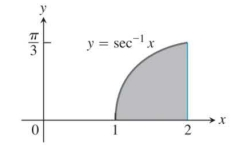
\includegraphics[width=4cm]{Selection_080.jpg} 
	\end{figure} 
	
	\item Determine o volume do sólido da região limitada pelos gráficos de $y = e^{-x^2}$, $y = 0$, $x = 0$ e $x = 1$ obtido com a rotação em torno do eixo y.
	
	\item Determine o volume do sólido da região limitada pelos gráficos de $y = e^{x/2}$, $y = 1$, $x = \ln 3$ obtido com a rotação em torno do eixo x.
     
     \item Você é o encarregado de projetar um peso de latão para prumo que pesará aproximadamente 190 $g$, e decide concebê-lo como o sólido de revolução mostrado abaixo. Determine o volume do peso. Se você especificar um latão com densidade 8,5 $g/cm^3$, qual será o peso em gramas do prumo? (arredonde para o inteiro mais próximo). 
     
    \begin{figure}[h]	
	\centering % para centralizarmos a figura	
	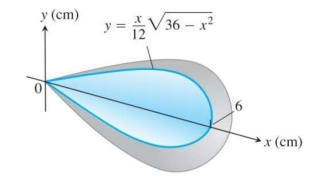
\includegraphics[width=6cm]{Selection_079.jpg} 
	\end{figure}
    
     \item Alguns dos pioneiros do cálculo, como Kepler e Newton, foram inspirados pelo problema de encontrar os volumes de barris de vinho. (De fato, Kepler publicou um livro em 1615, \textit{Stereometria doliorum}, dedicado aos métodos para encontrar os volumes de barris.) Eles frequentemente aproximavam a forma dos lados por parábolas. 
     \begin{enumerate}
     \item Um barril com altura $A$ e raio máximo $R$ é construído pela rotação ao redor do eixo da parábola $y = R - cx^2$, $-h/2 \leq x \leq h/2$, onde $c$ é uma constante positiva. Mostre que o raio de cada extremidade do barril é $r = R - d$, onde $d = ch^2/4$.
     \item Mostre que o volume delimitado pelo barril é
     $$V = \displaystyle\dfrac{1}{3} \pi h \left(2R^2 + r^2 - \displaystyle\dfrac{2}{5}d^2\right)$$
     \end{enumerate}
     
     \item Calcule o comprimento de arco da parábola semicúbica $y^2 = x^3$ entre os pontos $(1 \mathrm{, } \ 1)$ e $(4 \mathrm{, } \ 8)$. 
		
	 \item Calcule o comprimento de arco da parábola $y^2 = x$ de $(0 \mathrm{, } \ 0)$ a $(1 \mathrm{, } \ 1)$.
	 \item Um vento contínuo sopra uma pipa para oeste. A altura da pipa acima do solo a partir da posição horizontal $x = 0$ até $x = 25$ é dada por $y = 50 - 0,1(x - 15)^2.$ Ache a distância percorrida pela pipa.
	 
	 \item Um falcão voando a 15 $m/s$ a uma altitude de 180 $m$ acidentalmente derruba sua presa. A trajetória parabólica de sua presa caindo é descrita pela equação
	 $$y = 180 - \displaystyle\dfrac{x^2}{45}$$
	 até que ela atinja o solo, onde $y$ é a altura acima do solo e $x$, a distância horizontal percorrida em metros. Calcule a distância percorrida pela presa do momento em que ela é derrubada até o momento em que ela atinge o solo. Expresse sua resposta com precisão de um décimo de metro. 
	 
	 \item Encontre o comprimento da curva
	 $$y = \displaystyle\int_1^x \sqrt{t^3 - 1} \ dt \mathrm{, } \ 1 \leq x \leq 4$$.
	 
	 \item Que curva é representada pelas seguintes equações paramétricas? 
	 
	 $$x = \cos t \quad \quad y = \sin t \quad \quad 0 \leq t \leq 2 \pi$$
	 
	 \item Esboce e identifique a curva definida pelas equações paramétricas
	 
	 $$x = t^2 - 2t \quad \quad y = t + 1$$
	 
	 \item Encontre a área sob um arco da ciclóide
	 $$x = r(\theta - \sin \theta) \quad \quad y = r(1 - \cos \theta)$$ 
	 
	 \item Encontre o comprimento de um arco da cicloide $x = r(\theta - \sin \theta)$, $y = r(1 - \cos \theta)$.
	 
	 \item Encontre a área da região sombreada das figuras abaixo:
	 
	 \begin{figure}[h]	
	\centering % para centralizarmos a figura	
	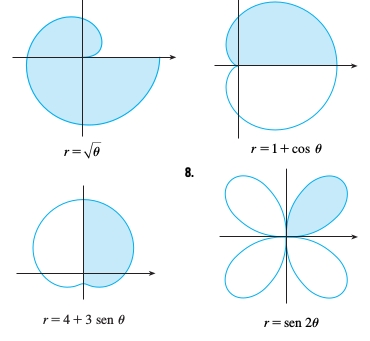
\includegraphics[width=7cm]{Selection_081.jpg} 
	\end{figure}
	 
	\item Calcule a área delimitada por um laço da rosácea de quatro pétalas $r = \cos 2\theta$.
	
	\item Calcule a área da região que está dentro do círculo $r = 3 \sin \theta$ e fora da cardioide $r = 1 + \sin \theta$.
	
	\item Esboce a curva e calcule a área delimitada por ela.
	\begin{enumerate}
	\item $r = 2 \sin \theta$.
	\item $r = 1 - \sin \theta$.
	\item $r = 3 + 2 \cos \theta$.
	\item $r = 4 + 3 \sin \theta$.
	\end{enumerate}
	
	\item Ao gravarem apresentações ao vivo, os engenheiros de som usam um padrão de captação em forma de cardióide, pois ele suprime o barulho da audiência. Suponha que o microfone esteja colocado a 4 $m$ da frente do palco (como na figura) e que o limite da região de captação ótima seja dado pelo cardioide $r = 8 + 8 \sin \theta$, onde $r$ é medido em metros e o microfone está no polo. Os músicos querem saber a área que eles terão no palco dentro da área de captação ótima do microfone. Responda a esta pergunta. 	
	\begin{figure}[h]	
	\centering % para centralizarmos a figura	
	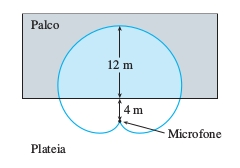
\includegraphics[width=5cm]{Selection_082.jpg} 
	\end{figure}
\end{enumerate}		
	
\end{document}